\begin{figure}[t]
	\centering
	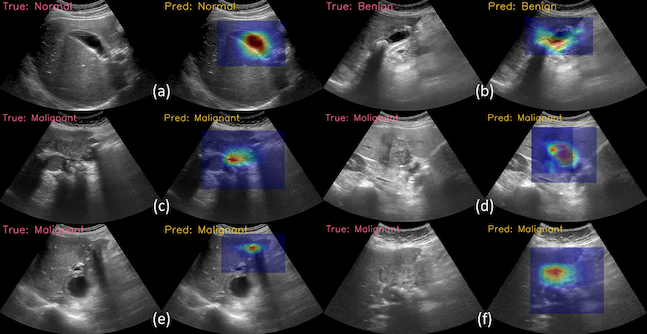
\includegraphics[width=0.7\linewidth]{figs/gbcnet/vis-s-1.png}
	\caption[Additional Grad-CAM visuals for GBCNet]{Sample Grad-CAM visuals of GBCNet with curriculum learning. (a) Normal, (b) Benign, and (c)--(f) Malignant samples.}
	\label{fig:supple-2}
\end{figure}

\begin{figure}[t]
	\centering
	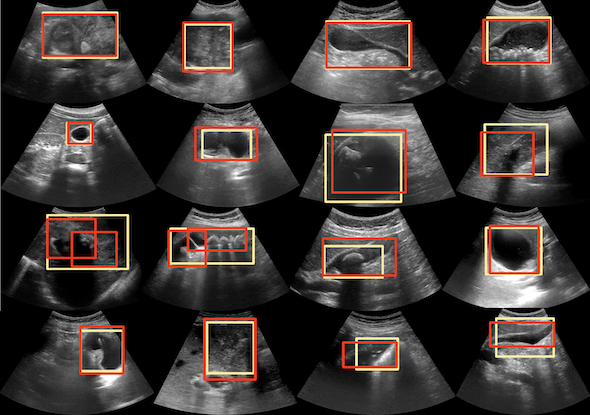
\includegraphics[width=0.7\linewidth]{figs/gbcnet/vis-s-0.png}
	\caption[Additional ROI visuals]{Sample visual results of RoI Detection models. First row - Faster-CNN, second row - YOLOv4, third row - Reppoints, and fourth row - CentripetalNet. Dark red is the ROI prediction by the model and light yellow is expert radiologists' perception of ROI.}
	\label{fig:supple-1}
\end{figure}

\section{Appendix}


\subsection{GradCAM Visuals for GBCNet}
\label{supp:cam_vis}
Figure \ref{fig:supple-2} shows the sample Grad-CAM visualizations of the predictions using GBCNet (ROI+MS-SoP) with curriculum learning. %The blue regions show the most vital regions used by the classifier during prediction. The classifier well emphasized the crucial visual cues during inference.  

\subsection{Candidate ROI Visuals}
\label{supp:roi_vis}
In figure \ref{fig:supple-1}, we show sample predictions of the GB region localization for different models. We also show the region of interest as perceived by the expert radiologists. The localization model is fairly accurate in capturing important regions of the USG image.

\subsection{Baseline Implementation Details}
%

\label{supp:impl}
\cref{tbl:configs} lists the configurations of all models which we have used. We trained on the Quadro P5000 16GB GPU. The table includes a brief description of the various stages of the network, input image sizes ($H\times W\times D$), the optimizer, relevant hyper-parameters such as learning rate, weight decay, momentum, batch size, and the number of training epochs/steps for the network. 
 \begin{table}[t]
\centering
\footnotesize
%\setlength{\tabcolsep}{4pt}
    \resizebox{ \linewidth}{!}{%
        \begin{tabular}{p{0.1\linewidth}p{0.42\linewidth}p{0.06\linewidth}p{0.2\linewidth}p{0.05\linewidth}p{0.06\linewidth}}
        \toprule[1.5pt]
        \textbf{Model} & \textbf{Description} & \textbf{Input Size} & \textbf{Optimizer} & \textbf{Batch size} & \textbf{Epochs/ Steps}
        \\ \midrule[0.75pt]
        YOLOv4 \cite{yolov4} & CSPDarknet53 backbone, PANet neck, anchor-based YOLO head. Total 162-layers. Backbone was frozen for first 800 step. Entire network was trainable thereafter. Single stage, anchor-based  & $608\times608\times3$ & SGD LR = 0.0001 momentum = 0.95 weight decay = 0.0005 & 64 & 3000 steps \\ \hline
        Reppoints \cite{reppoints} & Resnet-101 backbone, Group Normalization neck, and a reppoints head. Backbone was frozen for first 30 epochs, and entire network was trainable thereafter. Two-stage, anchor-free & $800 \times 1333 \times 3$ & SGD LR = 0.001 momentum = 0.9 weight decay = 0.0001 & 4 & 50 epochs \\ \hline
        Centripetal-Net \cite{centripetalnet} & HourglassNet-104 backbone. Enitre network was trainable. Anchor-free & $511 \times 511 \times 3$ & Adam LR = 0.0005 & 4 & 50 epochs \\ \hline
        ResNet \cite{resnet} & Resnet-50 used. All layers were trainable. LR decays by 10\% after every 5 epochs through a step LR scheduler. & $224\times224\times3$ & SGD LR = 0.005 momentum = 0.9 weight decay = 0.0005 & 16 & 100 epochs \\ \hline
        VGG \cite{vgg} & VGG-16 is used. All layers were trainable. LR decays by 10\% after every 5 epochs through a step LR scheduler. & $224\times224\times3$ & SGD LR = 0.005 momentum = 0.9 weight decay = 0.0005 & 16 & 100 epochs \\ \hline
        Inception \cite{inception} & Inception-V3 used. All layers were trainable. LR decays by 10\% after every 5 epochs through a step LR scheduler. & $299\times299\times3$ & SGD LR = 0.005 momentum = 0.9 weight decay = 0.0005 & 16 & 100 epochs \\ \hline
        RetinaNet \cite{retinanet} & Resnet-18-FPN used as backbone. All layers were trainable. & $512\times512\times3$ & Adam LR = 0.0001 & 8 & 50 epochs \\ \hline
        EfficientDet \cite{efficientdet} & EfficientNet-B4 used as backbone and BiFPN as feature network. All layers were trainable. & $1024\times1024\times3$ & Adam LR = 0.001 & 2 & 50 epochs \\ 
        \bottomrule
    \end{tabular}
    }
    \caption[Implementation details for the different baseline networks]{Implementation details for the different baseline networks used for classification and \gb localization.}
    \label{tbl:configs}
\end{table}





